%% Total contracts = 138
%% Total checks = 3708620
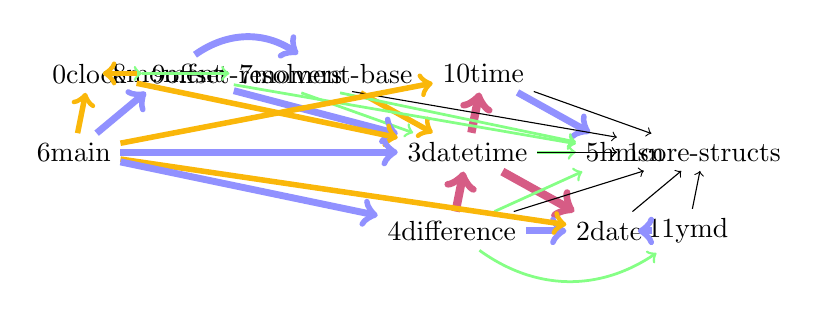
\begin{tikzpicture}

  \node (00)              {};
  \node (01) [below of=00,xshift=0.8cm] {\rkt{1}{core-structs}};
  \node (02) [below of=01,xshift=0.8cm] {};

  \node (10) [left of=00] {};
  \node (11) [left of=01] {\rkt{5}{hmsn}};
  \node (12) [left of=02] {\rkt{11}{ymd}};

  \node (20) [left of=10] {\rkt{10}{time}};
  \node (21) [left of=11] {};
  \node (22) [left of=12] {\rkt{2}{date}};

  \node (30) [left of=20] {};
  \node (31) [left of=21] {\rkt{3}{datetime}};
  \node (32) [left of=22] {};

  \node (40) [left of=30] {\rkt{7}{moment-base}};
  \node (41) [left of=31] {};
  \node (42) [left of=32] {\rkt{4}{difference}};

  \node (50) [left of=40] {\rkt{9}{offset-resolvers}};
  \node (51) [left of=41] {};
  \node (52) [left of=42] {};

  \node (60) [left of=50] {\rkt{8}{moment}};
  \node (61) [left of=51] {};
  \node (62) [left of=52] {};

  \node (70) [left of=60] {\rkt{0}{clock}};
  \node (71) [left of=61] {};
  \node (72) [left of=62] {};

  \node (81) [left of=71] {\rkt{6}{main}};

  %% -- edges
  %% gregor-structs
%% WARNING: no data for boundary 'core-structs.rkt' ==> 'gregor-structs.rkt'
  %% hmsn
%% WARNING: no data for boundary 'core-structs.rkt' ==> 'hmsn.rkt'
  \draw[->] (11) -- (01);
  %% ymd
%% WARNING: no data for boundary 'core-structs.rkt' ==> 'ymd.rkt'
  \draw[->] (12) -- (01);
  %% date
%% WARNING: no data for boundary 'gregor-structs.rkt' ==> 'date.rkt'
%% WARNING: no data for boundary 'core-structs.rkt' ==> 'date.rkt'
  \draw[->] (22) -- (01);
  \draw[->,blue!43!white, line width=2.5pt] (22) -- (12);
  %% time
%% WARNING: no data for boundary 'core-structs.rkt' ==> 'time.rkt'
  \draw[->] (20) -- (01);
%% WARNING: no data for boundary 'gregor-structs.rkt' ==> 'time.rkt'
  \draw[->,blue!43!white, line width=2.5pt] (20) -- (11);
  %% datetime
  \draw[->,purple!64!white, line width=3pt] (31) -- (20);
  \draw[->,purple!64!white, line width=3pt] (31) -- (22);
  \draw[->,green!48!white, line width=1pt] (31) -- (11);
%% WARNING: no data for boundary 'gregor-structs.rkt' ==> 'datetime.rkt'
%% WARNING: no data for boundary 'core-structs.rkt' ==> 'datetime.rkt'
  \draw[->] (31) -- (01);
  %% diff
%% WARNING: no data for boundary 'core-structs.rkt' ==> 'difference.rkt'
  \draw[->] (42) -- (01);
%% WARNING: no data for boundary 'gregor-structs.rkt' ==> 'difference.rkt'
  \draw[->,green!48!white, line width=1pt] (42) -- (11);
  \draw[->,green!48!white, line width=1pt] (42) edge[bend right=35] (12);
  \draw[->,blue!43!white, line width=2.5pt] (42) -- (22);
  \draw[->,purple!64!white, line width=3pt] (42) -- (31);
  %% moment-base
%% WARNING: no data for boundary 'gregor-structs.rkt' ==> 'moment-base.rkt'
  \draw[->,yellow!45!orange, line width=2pt] (40) -- (31);
  %% offset-resolvers
%% WARNING: no data for boundary 'core-structs.rkt' ==> 'offset-resolvers.rkt'
  \draw[->] (50) -- (01);
%% WARNING: no data for boundary 'gregor-structs.rkt' ==> 'offset-resolvers.rkt'
  \draw[->,green!48!white, line width=1pt] (50) -- (11);
  \draw[->,green!48!white, line width=1pt] (50) -- (31);
  \draw[->,green!48!white, line width=1pt] (50) -- (40);
  %% moment
%% WARNING: no data for boundary 'gregor-structs.rkt' ==> 'moment.rkt'
  \draw[->,green!48!white, line width=1pt] (60) -- (11);
  \draw[->,blue!43!white, line width=2.5pt] (60) -- (31);
  \draw[->,blue!43!white, line width=2.5pt] (60) edge[bend left=35] (40);
  \draw[->,green!48!white, line width=1pt] (60) -- (50);
  %% clock
%% WARNING: no data for boundary 'gregor-structs.rkt' ==> 'clock.rkt'
  \draw[->,yellow!45!orange, line width=2pt] (70) -- (31);
  \draw[->,yellow!45!orange, line width=2pt] (70) -- (60);
  %% main
%% WARNING: no data for boundary 'gregor-structs.rkt' ==> 'main.rkt'
  \draw[->,yellow!45!orange, line width=2pt] (81) -- (20);
  \draw[->,yellow!45!orange, line width=2pt] (81) -- (22);
  \draw[->,blue!43!white, line width=2.5pt] (81) -- (31);
  \draw[->,blue!43!white, line width=2.5pt] (81) -- (60);
  \draw[->,yellow!45!orange, line width=2pt] (81) -- (70);
  \draw[->,blue!43!white, line width=2.5pt] (81) -- (42);

\end{tikzpicture}
